\documentclass[11pt]{article}
\usepackage[margin=1in]{geometry}
\usepackage{amsmath,amssymb}
\usepackage[T1]{fontenc}
\usepackage{lmodern}
\usepackage{microtype}
\usepackage{graphicx}
\usepackage{caption}
\captionsetup{font=small,skip=5pt,hypcap=false}
\usepackage[hidelinks]{hyperref}
\setlength{\parskip}{3pt}
\setlength{\parindent}{1em}
\raggedbottom
\clubpenalty=10000
\widowpenalty=10000
\displaywidowpenalty=10000
\newcommand{\GRBUpper}{9.91\times10^{-28}}
\newcommand{\CrabUpper}{1.16\times10^{-26}}
\newcommand{\PKSUpper}{1.07\times10^{-26}}
\newcommand{\PlanckLength}{1.62\times10^{-35}}
\newcommand{\LengthGap}{6.13\times10^{7}}
\newcommand{\CoefficientGap}{3.76\times10^{15}}
\newcommand{\CountFactor}{1.41\times10^{31}}
\newcommand{\GRBPlanckDelay}{3.16\times10^{-15}}
\newcommand{\CrabPlanckDelay}{6.50\times10^{-23}}
\newcommand{\PKSPlanckDelay}{7.34\times10^{-16}}
\newcommand{\GRBHighestLag}{9.36\times10^{-1}}
\newcommand{\GRBHighestError}{4.31\times10^{-1}}

\title{Photon-Timing Tests of a Minimum-Distance\\Propagation Model}
\author{J. R. Landers}
\date{November 13, 2026}
\begin{document}
\maketitle
\begin{abstract}
This companion to \emph{Consequences of Minimum Distance in Mathematics and Physics} relates its lattice-wave formalism to three observational comparisons: LHAASO measurements of GRB 221009A, MAGIC measurements of the Crab pulsar, and H.E.S.S. measurements of PKS 2155--304. The work comprises an exploratory calculation from released LHAASO light curves, a recalculation of published Crab pulse-position summaries, and transformations of published propagation bounds for all three sources. The calibrated published analyses have not been independently reproduced. Their results constrain the effective interaction length to approximately $10^{-27}$--$10^{-26}$ m, conditional on photon dynamics, the quadratic regime, and source assumptions. They do not provide affirmative evidence for a minimum distance. Planck spacing with nearest-neighbor interactions predicts delays far below the sensitivity of these comparisons. We distinguish the spacing from the effective interaction length and quantify the improvement required to test that particular Planck-scale model.
\end{abstract}

\section{Purpose and scope}
The original exposition \cite{landers} separates a geometric hypothesis from a dynamical construction. A positive gap between distinct spatial positions restricts admissible triangles, repeated bisection, and continuous position-valued trajectories. It does not by itself determine how light propagates. The observational bridge is supplied by continuously evolving fields on a lattice and, subsequently, by the additional assumption that photon wave packets share their dispersion.

Here we review that bridge before presenting the three comparisons. These are reanalyses and interpretations of existing observations, rather than three new laboratory experiments. In particular, a timing feature in a released light curve is not automatically a propagation delay, and agreement with a published upper bound is not evidence that a distance gap exists. The distinction between independently computed diagnostics and transformed published results is maintained throughout.

\newpage
\section{From a position gap to a photon-delay coefficient}
Let physical positions form a metric space satisfying
\begin{equation}
 x\ne y\quad\Longrightarrow\quad d(x,y)\geq k>0.
\end{equation}
For the propagation model, specialize to $X=k\mathbb Z$ and take a scalar amplitude $u_n(t)$ with symmetric finite-range restoring interactions,
\begin{equation}\label{wave}
 \ddot u_n=\sum_{r=1}^{R}g_r(u_{n+r}-2u_n+u_{n-r}),
 \qquad g_r\geq0,
\end{equation}
with at least one nonzero coupling. This choice of positions and dynamics supplies assumptions beyond the metric gap. Plane waves give
\begin{equation}
 \omega^2(q)=4\sum_{r=1}^{R}g_r\sin^2(rqk/2).
\end{equation}
Define
\begin{equation}\label{length}
 c^2=k^2\sum_r g_r r^2,\qquad
 \Lambda^2=k^2\frac{\sum_r g_r r^4}{\sum_r g_r r^2}.
\end{equation}
At low wave number on the positive-frequency, right-moving branch,
\begin{equation}
 \omega=cq\left[1-\frac{\Lambda^2q^2}{24}+O(q^4)\right],
 \qquad
 v_g=c\left[1-\frac{\Lambda^2q^2}{8}+O(q^4)\right].
\end{equation}
For each fixed finite-range model this is an asymptotic expansion. A sufficient condition for using the displayed term across an observed band is $qRk\ll1$. A small fitted leading coefficient alone need not guarantee this condition for arbitrarily distant, weak couplings.

Writing $w_r=g_r r^2/\sum_s g_s s^2$ gives
\begin{equation}\label{gapbound}
 \Lambda^2=k^2\sum_r w_r r^2\geq k^2.
\end{equation}
Thus $k$ is the spacing, while $\Lambda$ is a weighted interaction length. They coincide for nearest-neighbor interactions. Positive longer-range couplings increase the leading coefficient; allowing negative couplings can cancel it, as the original exposition illustrates. The bound used here therefore applies to the specified positive-coupling class in its quadratic regime.

Now assume photons inherit this dispersion and $E=\hbar\omega$. To leading order,
\begin{equation}\label{velocity}
 \frac{v_g(E)}{c}=1-\frac{\Lambda^2E^2}{8\hbar^2c^2}+O(E^4).
\end{equation}
For observed energies $E_{h,0}>E_{l,0}$ from redshift $z_s$, the cosmological embedding used in the original paper gives
\begin{align}
 K_2(z_s)&=\int_0^{z_s}\frac{(1+z)^2}{H(z)}\,dz,\\
 \Delta t_{\rm prop}&\simeq B\,(E_{h,0}^2-E_{l,0}^2)K_2(z_s),
 \qquad B=\frac{\Lambda^2}{8(\hbar c)^2}\geq0.\label{delay}
\end{align}
This assumes constant physical $\Lambda$ in the cosmological rest frame and the usual leading-order photon redshift. For the Galactic Crab pulsar, replace $K_2$ by $D/c$, where $D$ is its distance.

The conventional subluminal quadratic parametrization is $v_g/c\simeq1-\tfrac32(E/E_{\rm QG,2})^2$. Matching it to Eq.~\eqref{velocity} gives
\begin{equation}\label{conversion}
 E_{\rm QG,2}=\frac{\sqrt{12}\,\hbar c}{\Lambda}.
\end{equation}
A published lower limit on this energy scale becomes an upper limit on $\Lambda$; Eq.~\eqref{gapbound} then bounds $k$. The conversion preserves the published statistical construction and its assumptions. It is not a new confidence calculation. Signed delay estimators may take negative values even though this model requires $B\geq0$; such values must not be converted into an imaginary physical length.

An observed lag also contains source emission and instrumental contributions. Without restrictions on these contributions, a single source cannot isolate $B$: an arbitrary intrinsic lag could imitate or offset the predicted effect. All physical limits below inherit the applicable source and detector assumptions.

The construction is one-dimensional. Applying it to an astronomical sightline assumes its effective propagation law holds along that direction. A common coefficient across different sightlines would require an isotropic extension or a specified angular dependence; neither a three-dimensional electromagnetic theory nor its directional response has yet been derived. The source limits below are therefore presented individually.

\section{Three observational comparisons}
\subsection{LHAASO: GRB 221009A}
The released WCDA light curves \cite{lhaasodata} permit a new exploratory cross-correlation calculation. We used ten channels over 232--400 s after the trigger, with 0.1 s bins, containing 54,767 ON events and an estimated 12,107.75 background events. A Gaussian plus constant was fitted to each correlation peak against the lowest channel over a fixed $\pm10$ s interval. Five hundred joint Poisson resamples of the ON and OFF histograms retained covariance from the shared reference.

The highest-channel lag was $0.936\pm0.431$ s. Changing the peak-fit interval to $\pm8$ or $\pm15$ s changed it to 0.752 or 1.148 s. These statistical errors omit response-overlap and spectral-evolution corrections. The highest and lowest channels have median energies 1.601 and 0.354 TeV; their true-energy distributions overlap. The feature is therefore an uncorrected timing diagnostic, not a photon-propagation detection.

For physical inference we use the published, bias-corrected result \cite{lhaaso}. Its quadratic parameter is
\begin{equation}
 \eta_2=10^{-15}\left(\frac{E_{\rm Pl}}{E_{\rm QG,2}}\right)^2
       =\frac{10^{-15}}{12}\left(\frac{\Lambda}{\ell_P}\right)^2.
\end{equation}
Here $\ell_P=\sqrt{\hbar G/c^3}$ and $E_{\rm Pl}=\hbar c/\ell_P$. The reported maximum-likelihood best fit is 0.01, with a 95\% interval $[-0.31,0.32]$, consistent with zero. The uncorrected value 0.20 and estimated bias 0.19 demonstrate why the correction matters. The rounded published scale limit $E_{\rm QG,2}>6.9\times10^{11}$ GeV gives $\Lambda<\GRBUpper$ m. Using the rounded interval endpoint instead gives $1.00\times10^{-27}$ m; the calibrated alternative gives approximately $9.5\times10^{-28}$ m. These differences reflect different published constructions and rounding. We have not repeated their full fit or calibration.

\newpage
\subsection{MAGIC: the Crab pulsar}
The published pulse positions \cite{crab} allow a summary calculation, though the original event-and-response sample was not located. Multiplying phase differences by a 33.7 ms period gives
\begin{center}
\begin{tabular}{lrrr}
\hline
Representative energies & Lag & Statistical error & Systematic error\\
(GeV) & ($\mu$s) & ($\mu$s) & ($\mu$s)\\ \hline
75 versus 770 & 175 & 165 & 101\\
465 versus 770 & 10 & 263 & 101\\ \hline
\end{tabular}
\end{center}
Adding the reported errors in quadrature gives 194 and 282 $\mu$s, respectively; both differences are compatible with zero. This illustrative treatment does not recalibrate coverage. The comparisons share a high-energy band, and the lower bands can involve different emission physics. They are not independent measurements of one propagation coefficient. Moreover, band means do not specify the second energy moments required for a response-integrated quadratic prediction.

We therefore take the full published profile-likelihood bound, including the reported systematics, rather than construct a new bound from the two peak differences. Its $E_{\rm QG,2}>5.9\times10^{10}$ GeV at 95\% confidence gives $\Lambda<\CrabUpper$ m. This is approximately 12 times weaker in length than the LHAASO result, but concerns a different source class and emission mechanism. It neither establishes a lag nor reproduces the original likelihood fit.

\subsection{H.E.S.S.: PKS 2155--304}
For the July 28, 2006 flare, the published final quadratic coefficient is \cite{pks}
\begin{equation}
 \tau_q=1.7\pm6.3_{\rm stat}\pm6.6_{\rm sys}\
 \mathrm{s\,TeV^{-2}},\qquad
 \Delta t=\tau_q(E_h^2-E_l^2)
\end{equation}
when energies are expressed in TeV. The combined illustrative error is $9.12$ s\,TeV$^{-2}$, placing the central value about 0.19 standard deviations from zero. The narrower error read directly from the likelihood curve is not the final calibrated error. The published 95\% scale limit $E_{\rm QG,2}>6.4\times10^{10}$ GeV gives $\Lambda<\PKSUpper$ m.

We also inspected the public H.E.S.S. DR1 event-and-response archive \cite{hessrelease}. It covers later flare nights, July 29--30, rather than this July 28 sample. Its terms restrict it to tool development and prohibit new scientific publications or source claims derived from those files. Separate private tool diagnostics are retained in the analysis workspace; their numerical outcomes and figures are not used here as scientific results. The comparison above is based exclusively on the published timing measurement and limit. We have not reproduced that event-level fit.

\clearpage
\section{What the bounds mean in this formalism}
Table~\ref{tab:bounds} uses the same conversion for all three published limits. They are individual 95\% bounds under their respective analyses; the table is not a joint confidence region. Their nuisance models and systematics differ, so combining only the quoted endpoints would not yield a calibrated combined limit.
\par\medskip\noindent
\begin{minipage}{\linewidth}
\centering
\small
\begin{tabular}{lcc}
\hline
Observation & Published $E_{\mathrm{QG},2}$ lower limit & Translated $\Lambda$ upper limit \\
 & (GeV) & (m) \\ \hline
LHAASO: GRB 221009A & $6.90\times10^{11}$ & $9.91\times10^{-28}$ \\
MAGIC: Crab pulsar & $5.90\times10^{10}$ & $1.16\times10^{-26}$ \\
H.E.S.S.: PKS 2155--304 & $6.40\times10^{10}$ & $1.07\times10^{-26}$ \\
\hline
\end{tabular}

\captionof{table}{Conditional bounds on the effective interaction length from published quadratic subluminal scale limits. The LHAASO entry uses its rounded maximum-likelihood scale bound.}\label{tab:bounds}
\end{minipage}
\par\medskip\noindent
\begin{minipage}{\linewidth}
\centering
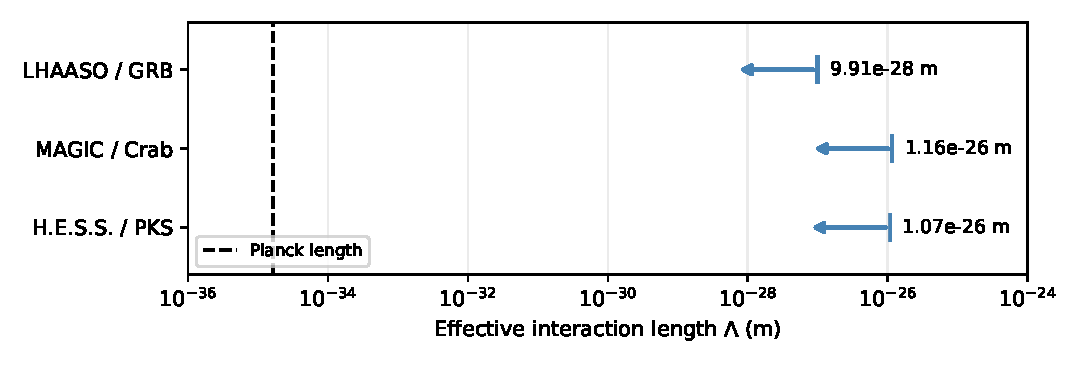
\includegraphics[width=.85\linewidth]{figures/length_bounds.pdf}
\captionof{figure}{Translated individual upper bounds; leftward arrows indicate the permitted direction. The dashed line marks $\ell_P$. The arrow lengths are graphical, not lower limits or probability distributions. All three bounds are far above Planck spacing.}\label{fig:bounds}
\end{minipage}
\par\medskip

The strongest of these comparisons gives $k\leq\Lambda\lesssim10^{-27}$ m. This condition disfavors larger spacings within the stated propagation model and its quadratic regime. It does not demonstrate that Euclidean constructions or continuous positions exist below $10^{-27}$ m: photon timing has not tested their existence. Nor does it reach below the Planck length, which is $\ell_P\simeq\PlanckLength$ m.

The observations remain compatible with $k=\ell_P$. They also permit finer spacings and a vanishing observable coefficient in continuum propagation. Compatibility is not affirmative support. A positive physical claim would require a propagation signature distinguished from source and instrument effects, ideally a common coefficient across sources after their distance factors are included. Even that would support the dispersion law before establishing a particular microscopic geometry.

There is an additional distinction within the lattice class. Setting $k=\ell_P$ does not force $\Lambda=\ell_P$; the latter specifies nearest-neighbor interactions. Let
\begin{equation}
 R_{\rm eff}=\sqrt{\sum_r w_r r^2},\qquad \Lambda=kR_{\rm eff}.
\end{equation}
At Planck spacing the LHAASO comparison constrains $R_{\rm eff}$ to roughly $6\times10^7$ lattice steps, if the observed energies remain in the quadratic regime. Thus some long-interaction models can be constrained even when the spacing is Planckian. This does not convert the bound into a direct spatial-resolution measurement.

\newpage
\section{The sensitivity gap and the next question}
The particularly difficult benchmark is $k=\Lambda=\ell_P$. The predicted delays calculated with the same formalism are
\begin{center}
\begin{tabular}{lll}
\hline
Source & Representative observed energies & Planck nearest-neighbor delay\\ \hline
GRB 221009A & 0.2 versus 7 TeV & $\GRBPlanckDelay$ s\\
Crab pulsar & 465 versus 770 GeV & $\CrabPlanckDelay$ s\\
PKS 2155--304 & 0.25 versus 4 TeV & $\PKSPlanckDelay$ s\\ \hline
\end{tabular}
\end{center}
These illustrate the model's scale; energy endpoints or representative means are not substitutes for the detector response in a fit. For the GRB we use $z=0.151$, $H_0=67.36$ km\,s$^{-1}$\,Mpc$^{-1}$ and $\Omega_m=0.315$. For PKS we retain the original analysis's $z=0.116$, $H_0=2.3\times10^{-18}$ s$^{-1}$ and $\Omega_m=0.3$. For the Crab we use its nominal distance of 2 kpc. Keeping the distinct assumptions explicit avoids implying a common cosmological refit.

The LHAASO length limit is about $\LengthGap$ Planck lengths. Because the leading delay is proportional to $\Lambda^2$, the corresponding gap in coefficient sensitivity is approximately $\CoefficientGap$. A somewhat larger telescope or another weakly constraining source cannot by itself close this gap.

To see the scaling, let $\sigma_{\Delta t}$ characterize an attainable propagation-delay uncertainty for a fixed energy lever arm and distance factor. Equation~\eqref{delay} gives schematically
\begin{equation}
 \Lambda_{\rm sens}\sim\hbar c\sqrt{
 \frac{8\sigma_{\Delta t}}{K_2(E_h^2-E_l^2)}}.
\end{equation}
If independent photon statistics alone gave $\sigma_{\Delta t}\propto N^{-1/2}$ with all other properties fixed, then $\Lambda_{\rm sens}\propto N^{-1/4}$. Closing the displayed length gap by this mechanism alone would require a count increase of order $\CountFactor$. This is an idealized scaling argument, not a forecast: evolving source structure and systematic errors also limit inference. Higher energies and sharper, well-understood features help, but their availability must be demonstrated observationally.

The three comparisons therefore establish the current task more clearly than they establish new physics. Further timing sources are useful for controlling source-specific effects and checking a common coefficient, while the nearest-neighbor Planck benchmark requires much higher sensitivity or a different observable derived from the model. Strong limits on polarization rotation, quantum commutators, or geometrical noise cannot be imported without the corresponding predictions. A natural subsequent question is whether an interacting photon--matter extension yields an experimentally accessible signature in high-energy photon interactions. That derivation is deferred; it is not assumed in any result of this note.

\newpage
\appendix
\section{Computational record}
The accompanying workspace retains the scripts and numeric outputs. The LHAASO calculation is recorded in \texttt{analysis/fit\_ccf.py} and \texttt{analysis/ccf\_results.json}; published-bound transformations are in \texttt{analysis/translated\_bounds.json}. The Crab calculation is in \texttt{analysis/crab/}, and the PKS published comparison and separately labeled tool work are in \texttt{analysis/pks2155/}.

Within this note's folder, \texttt{prepare\_results.py} reads the saved JSON files, checks the scale-to-length identity, and generates the table, numerical macros, figure, and \texttt{provenance.json} with input hashes. It performs no new inference. The quoted raw LHAASO lag errors remain approximate bootstrap errors. Quadrature error combinations for Crab and PKS are illustrative. No new propagation-only confidence interval, full calibrated likelihood reproduction, or joint cross-source confidence limit is claimed.

\begin{thebibliography}{9}
\small
\bibitem{landers} J. R. Landers, \emph{Consequences of Minimum Distance in Mathematics and Physics}, unpublished manuscript, November 13, 2026.
\bibitem{lhaaso} Z. Cao et al. (LHAASO Collaboration), Stringent tests of Lorentz invariance violation from LHAASO observations of GRB 221009A, \emph{Physical Review Letters} \textbf{133} (2024), 071501. \href{https://doi.org/10.1103/PhysRevLett.133.071501}{doi:10.1103/PhysRevLett.133.071501}.
\bibitem{lhaasodata} LHAASO Collaboration, data accompanying the GRB 221009A Lorentz-invariance study. \href{https://doi.org/10.12402/opendata/LHAASO/20240829100037}{doi:10.12402/opendata/LHAASO/20240829100037}.
\bibitem{crab} M. L. Ahnen et al. (MAGIC Collaboration), Constraining Lorentz invariance violation using the Crab Pulsar emission observed up to TeV energies by MAGIC, \emph{Astrophysical Journal Supplement Series} \textbf{232} (2017), 9. \href{https://doi.org/10.3847/1538-4365/aa8404}{doi:10.3847/1538-4365/aa8404}.
\bibitem{pks} A. Abramowski et al. (H.E.S.S. Collaboration), Search for Lorentz invariance breaking with a likelihood fit of the PKS 2155--304 flare data taken on MJD 53944, \emph{Astroparticle Physics} \textbf{34} (2011), 738--747. \href{https://doi.org/10.1016/j.astropartphys.2011.01.007}{doi:10.1016/j.astropartphys.2011.01.007}.
\bibitem{hessrelease} H. Abdalla et al. (H.E.S.S. Collaboration), \emph{H.E.S.S. first public test data release}, release documentation (2018). \href{https://arxiv.org/abs/1810.04516}{arXiv:1810.04516}. Cited for data provenance and scope; no scientific results derived from its restricted test events are presented here.
\end{thebibliography}
\end{document}
